\documentclass[$if(fontsize)$$fontsize$,$endif$$if(lang)$$lang$,$endif$$if(papersize)$$papersize$,$endif$]{acm_proc_article-sp}

% from Pandoc standard LaTeX templates
\usepackage[T1]{fontenc}
\usepackage{lmodern}
\usepackage{amssymb,amsmath}
\usepackage{ifxetex,ifluatex}
\usepackage{fancyvrb,relsize}
\usepackage{parskip}
\usepackage{fixltx2e} % provides \textsubscript
% use upquote if available, for straight quotes in verbatim environments
\IfFileExists{upquote.sty}{\usepackage{upquote}}{}
\ifnum 0\ifxetex 1\fi\ifluatex 1\fi=0 % if pdftex
  \usepackage[utf8]{inputenc}
$if(euro)$
  \usepackage{eurosym}
$endif$
\else % if luatex or xelatex
  \usepackage{fontspec}
  \ifxetex
    \usepackage{xltxtra,xunicode}
  \fi
  \defaultfontfeatures{Mapping=tex-text,Scale=MatchLowercase}
  \newcommand{\euro}{€}
$if(mainfont)$
    \setmainfont{$mainfont$}
$endif$
$if(sansfont)$
    \setsansfont{$sansfont$}
$endif$
$if(monofont)$
    \setmonofont{$monofont$}
$endif$
$if(mathfont)$
    \setmathfont{$mathfont$}
$endif$
\fi
% use microtype if available
\IfFileExists{microtype.sty}{\usepackage{microtype}}{}
$if(geometry)$
\usepackage[$for(geometry)$$geometry$$sep$,$endfor$]{geometry}
$endif$
$if(natbib)$
\usepackage{natbib}
\bibliographystyle{plainnat}
$endif$
$if(biblatex)$
\usepackage{biblatex}
$if(biblio-files)$
\bibliography{$biblio-files$}
$endif$
$endif$
$if(listings)$
\usepackage{listings}
$endif$
$if(lhs)$
\lstnewenvironment{code}{\lstset{language=Haskell,basicstyle=\small\ttfamily}}{}
$endif$
$if(highlighting-macros)$
$highlighting-macros$
$endif$
$if(verbatim-in-note)$
\usepackage{fancyvrb,relsize}
$endif$
$if(tables)$
% don't use longtable, because of two-column mode!
$endif$
$if(graphics)$
\usepackage{graphicx}
% We will generate all images so they have a width \maxwidth. This means
% that they will get their normal width if they fit onto the page, but
% are scaled down if they would overflow the margins.
\makeatletter
\def\maxwidth{\ifdim\Gin@nat@width>\linewidth\linewidth
\else\Gin@nat@width\fi}
\makeatother
\let\Oldincludegraphics\includegraphics
\renewcommand{\includegraphics}[1]{\Oldincludegraphics[width=\maxwidth]{#1}}
$endif$
\ifxetex
  \usepackage[setpagesize=false, % page size defined by xetex
              unicode=false, % unicode breaks when used with xetex
              xetex]{hyperref}
\else
  \usepackage[unicode=true]{hyperref}
\fi
\urlstyle{same}  % don't use monospace font for urls
$if(links-as-notes)$
% Make links footnotes instead of hotlinks:
\renewcommand{\href}[2]{#2\footnote{\url{#1}}}
$endif$
$if(strikeout)$
\usepackage[normalem]{ulem}
% avoid problems with \sout in headers with hyperref:
\pdfstringdefDisableCommands{\renewcommand{\sout}{}}
$endif$
\setlength{\parindent}{0pt}
\setlength{\parskip}{6pt plus 2pt minus 1pt}
\setlength{\emergencystretch}{3em}  % prevent overfull lines
$if(numbersections)$
\setcounter{secnumdepth}{5}
$else$
\setcounter{secnumdepth}{0}
$endif$
$if(verbatim-in-note)$
\VerbatimFootnotes % allows verbatim text in footnotes
$endif$
$if(lang)$
\ifxetex
  \usepackage{polyglossia}
  \setmainlanguage{$mainlang$}
\else
  \usepackage[$lang$]{babel}
\fi
$endif$
$for(header-includes)$
$header-includes$
$endfor$

\DefineVerbatimEnvironment{verbatim}{Verbatim}{frame=single,framerule=0.5pt,framesep=0.4em,numbers=none,numbersep=0.5em,stepnumber=1,numberblanklines=true,fontsize=\relsize{-3}}

\pagenumbering{arabic}

\begin{document}

$if(title)$\title{$title$}$endif$
$if(subtitle)$\subtitle{$subtitle$}$endif$
$if(numberofauthors)$\numberofauthors{$numberofauthors$}$endif$

\author{
$for(author)$
  %\alignauthor 
  $author.name$
  $if(author.refaddr)$
    \\
    $for(author.refaddr)$
      \affaddr{$author.refaddr$}\\
    $endfor$
  $endif$
  $if(author.email)$\email{$author.email$}$endif$
  \and
$endfor$
}

%%$if(permission)$
%%\permission{
%%    $permission$
%%    $if(doi)$\\http://dox.doi.org/$doi$$endif$
%%}
%%$endif$


%%$if(conference.short)$
%%\conferenceinfo{CONF-INFO $conference.short$}{$conference.full$}
%%$endif$

\conferenceinfo{Bloomberg Data For Good Exchange Conference, }{28 Sep 2015.}

\permission{http://dox.doi.org/xxx-xxx-xxx}

$if(license)$
%%\copyrightetc{\includegraphics{by-nc.eps} $license$ $for(author)$ $author.name$ $endfor$ $conference_date$}
\copyrightetc{\href{https://creativecommons.org/licenses/by/4.0/}{\includegraphics{by.eps}}}
$endif$


$if(additionalauthors)$\additionalauthors{$additionalauthors$}$endif$

\date{$date$}

$if(title)$\maketitle$endif$

$if(abstract)$
\begin{abstract}
$abstract$
\end{abstract}
$endif$

%%$for(category)$
%%$category$
%%$endfor$

%%$if(terms)$\terms{$terms$}$endif$
%%$if(keywords)$\keywords{$keywords$}$endif$

$body$

\end{document}
